\chapter{Metodología del Trabajo}
\label{chap:metodologia}
El desarrollo de este proyecto se basó en una metodología completamente computacional, debido a que el trabajo principal fue la realización de múltiples simulaciones y la creación e implementación de códigos y programas para su análisis. La metodología propuesta y usada a lo largo del semestre se puede resumir en la Figura \ref{fig:meto} en donde se pueden ver las diferentes etapas del proyecto. En la primera etapa se consultó el material bibliográfico disponible tanto para la generación de simulaciones a través de Gadget-2 \cite{gadget}, así como para la comprensión de los conocimientos básicos para el desarrollo del proyecto, explicados en el Capítulo \ref{chap:marco}. 

\begin{figure}[H]
	\centering
	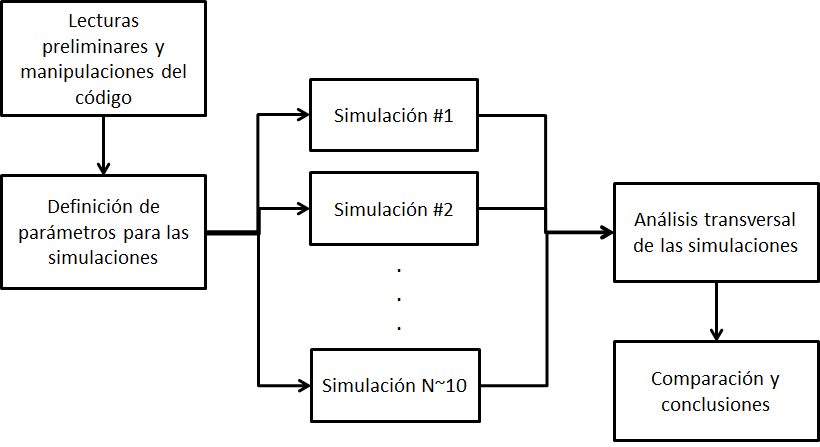
\includegraphics[width=11cm]{Metodologia/metodologia.png}
	\caption{Metodología de trabajo}
	\label{fig:meto}
\end{figure}

Una vez instaladas todas las librerías y códigos necesarios en el cluster de física, se procedió a realizar una serie de simulaciones preliminares. Éstas tenían como objetivo principal observar la dinámica del código, sus posibles errores, medir el tiempo de computación y sobretodo tener una muestra de los archivos exportados en cada simulación para poder analizarlos, ver su estructura y la información que contenían y en base a ello comenzar a escribir códigos de análisis que servirían para las simulaciones grandes. Estas primeras simulaciones se basaban en cajas cúbicas periódicas de lado de $150Mpc$ y contenían $128^3$ y $256^3$ partículas.

Una vez realizadas todas las pruebas preliminares se prepararon las condiciones iniciales para las simulaciones definitivas, las cuales por restricción de tiempo y recursos computacionales se fijaron a un cubo de $500Mpc$ de lado con un total de $512^3$ partículas. Dado el número de partículas, el tiempo de simulación comenzó a aumentar en un factor de 8, así que mientras que las simulaciones de $128^3$ partículas tomaban alrededor de 3 horas, las siguientes tomaron un día entero. Desafortunadamente al momento de correr las simulaciones definitivas, estas no fallaron por falta de memoria en el cluster de la universidad, por más que se corrieran en los 56 procesadores no lograba tener registro de todas las partículas. 


El análisis realizado a los resultados de las simulaciones tuvo dos vertientes principales: análisis por halos de materia oscura y análisis de fluctuaciones de densidades. De igual manera se generaron dos secuencias de código independientes para cumplir con ambos propósitos. Para la primera se hizo uso de un código existente para la búsqueda de halos por medio del algoritmo FoF y posteriormente se usó la información de los halos, como por ejemplo sus centros de masa y velocidades respectivas, tanto para un análisis intrínseco de cada simulación como para un análisis transversal entre las simulaciones. Para la segunda vertiente se calculó el campo de densidades de cada una de las simulaciones para realizar un análisis del espectro de fluctuaciones en cada caso. Para cada una de las simulaciones finales se varió la proporción de materia y energía oscura en el universo.

\section{Cronograma de Trabajo}
A continuación, en la Tabla \ref{tab:crono} se muestra el plan de trabajo propuesto para la realización del proyecto, junto con la distribución de tiempo establecida para la realización de cada una de las tareas.

\begin{table}[H]
	\centering
	\begin{tabular}{>{\centering}p{5cm}cp{7.5cm}}
		\hline \hline
		\textbf{Actividad} & \textbf{Duración} & \textbf{Descripción} \\
		\hline
		Lectura de Bases teóricas & 2 semanas & Revisión bibliográfica acerca de la composición del universo y los parámetros que definen su evolución.\\
		Lectura e instalación del código & 2 semanas & Instalación de librerías y entornos necesarios. Familiarización con los métodos de simulación y los códigos y lenguajes a usar.\\
		Simulaciones preliminares & 3 semanas & Realización de simulaciones de bajo nivel, observando archivos exportados y comportamiento.\\
		Simulaciones definitivas & 4 semanas & Adquisición de datos definitivos de análisis con simulaciones de alto nivel computacional.\\
		Análisis de simulaciones y creación de códigos& 3 semanas & Creación de programas de análisis en base a los formatos de exportación de Gadget-2 y generación de estadísticas y comparaciones.\\
		Redacción de documento & 3 semanas & Recoger los datos obtenidos y resultados de los análisis para redactar documento final.\\		
		\hline
	\end{tabular}
	\caption[Cronograma de Trabajo]{Cronograma de Trabajo \footnotemark}
	\label{tab:crono}
\end{table}

\footnotetext{La realización de las tareas no fue secuencial y los tiempos mostrados se sobrelapan durante el semestre}



